\documentclass{article}

\newcommand{\question}[2]{{\noindent \bf #1} #2}
\usepackage[french]{babel}
\usepackage{hyperref}
\usepackage{amsmath}
\usepackage{verbatim}
\usepackage{shortvrb}
\ifpdf \usepackage[pdftex]{graphicx} \pdfcompresslevel=9

\MakeShortVerb{|}

\title{TP |Unity|: \\ Cin\'ematique inverse avec l'algorithme CCD }
\date{\today}
\author{Steve Tonneau\\ IRISA}

\begin{document}
\maketitle

\section*{Introduction}
Ce TP propose de traiter un probl\`eme concret, r\'ecurent dans le domaine de l'animation, celui de la 
cin\'ematique inverse. La partie \ref{problem} de ce document est consacr\'ee \`a la description du probl\`eme. La
partie \ref{algo} est consacr\'ee \`a la pr\'esentation de l'algorithme CCD (pour Cyclic Coordinate Descent), tr\`es utilis\'e,
en particulier dans le domaine du jeu vid\'eo, pour r\'esoudre le probl\`eme de cin\'ematique inverse.
La partie \ref{implementation} a pour 
but de guider les \'etudiants dans l'impl\'ementation de l'algorithme CCD.
On l'impl\'ementera d'abord en 2, puis en 3 dimensions.

\subsection*{Public concern\'e}
Ce tp s'adresse \`a des \'etudiants en premi\`ere ann\'ee d'informatique. Il requiert une connaissance
minimale du moteur |Unity| 3d \footnote{\href{http://unity3d.com/unity}{http://unity3d.com/unity.}} (Menus, syst\`eme de scripts).
Les signatures des m\'ethodes utilis\'ees sont pr\'esent\'ees en C\#, mais il est facile de les transposer pour les langages Boo et javascript
\'egalement accept\'es sous |Unity|. Aussi il est \'egalement n\'ecessaire d'avoir des connaissances dans un de ces langages cibles.

Pour comprendre et impl\'ementer l'algorithme CCD sous |Unity|, des connaissances math\'ematiques de niveau lyc\'ee sont n\'ecessaires.

\subsection*{Dur\'ee}
TODO 

\subsection*{Mat\'eriel}
Un squelette de projet est disponible \`a l'adresse TODO. Il n\'ecessite une version d'|Unity| (gratuite ou pro) sup\'erieure ou \'egale \`a la version 4.1. \\

Le projet comprend:
\begin{itemize}
	\item Une sc\`ene |testScene.unity|. Elle comprend elle-m\^eme:
		\begin{itemize} 
			\item Une hi\'erarchie de sph\`eres qui servira de cha\^ine cin\'ematique pour l'exercice; la premi\`ere sph\`ere s'appelle |root|, la derni\`ere |effector|;
			\item Un cube |target|, qui repr\'esentera la cible \`a atteindre par notre cha\^ine cin\'ematique.
		\end{itemize}
	\item Deux squelettes |CCD2d.cs| et |CCD3d.cs|, qu'il va falloir modifier;
	\item Un script |TargetController.cs|, d\'ej\`a impl\'ement\'e, qui permet de contr\^oler la cible au clavier.
\end{itemize}

\section{Probl\'ematique: La cin\'ematique inverse}
\label{problem}

\subsection{Exemple introductif: r\'eglage de l'heure}
\label{montreex}
Consid\'erons la montre \`a gauche de la figure \ref{watch}:
\begin{figure}[htb]
  \centering
    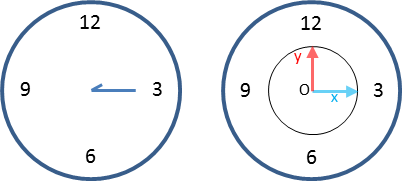
\includegraphics[]{watch2}
  \caption{
          \textit{A gauche: Une montre indiquant 2h15. A droite: la m\^eme montre munie d'un rep\`ere cart\'esien $(\vec{Ox}, \vec{Oy})$.}}
		   \label{watch}
\end{figure}

\subsubsection*{Cin\'ematique directe}
Nous munissons notre montre d'un rep\`ere cart\'esien $(\vec{Ox}, \vec{Oy})$ (figure \ref{watch}, droite), dans lequel la longueur
de la grande aiguille vaut 1.
Nous appelons l'extr\'emit\'e ext\'erieure de l'aiguille \textbf{effecteur}. On observe en fait que l'effecteur se d\'eplace
le long du cercle trigonom\`etrique associ\'e au rep\`ere $(\vec{Ox}, \vec{Oy})$. \\
Ce d\'eplacement est r\'ealis\'e par une rotation d'un angle $\theta$ autour d'un troisi\'eme axe $\vec{Oz} = \vec{Ox} \wedge \vec{Oy}$, qui prend
son origine en $O$.

On d\'efinit donc la fonction \textit{f}, telle que
 \begin{displaymath}  
f(\theta) =  \begin{pmatrix}
cos(\theta) \\
sin(\theta)
\end{pmatrix}
 \end{displaymath}
avec \begin{math} \theta \in [-2\pi, 2\pi[ \end{math}. \\

Gr\^ace \`a $f$ on peut conna\^itre la position de l'effecteur de la grande aiguille en fonction de l'angle $\theta$. Par exemple, si $\theta = -\pi / 2$,
l'effecteur est \`a la position $\begin{pmatrix}
0 \\
-1
\end{pmatrix}$, comme montr\'e sur la figure \ref{2h30}

\begin{figure}[htb]
  \centering
    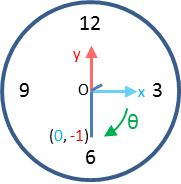
\includegraphics[]{watchrotcart}
  \caption{
          \textit{Si on choisit $\theta = -\pi / 2$, la montre indique maintenant 2h30.}}
		   \label{2h30}
\end{figure}

Ceci constitue un exemple de \textbf{cin\'ematique directe}: \`a partir d'un angle $\theta$, nous calculons une position
$\begin{pmatrix} x \\ y \end{pmatrix}$.

\subsubsection*{Cin\'ematique inverse}
On consid\`ere le probl\`eme inverse:
On souhaite r\'egler l'heure \`a 2h30,  c'est \`a dire que l'extr\'emit\'e de la grande aiguille aie pour coordonn\'ees $\begin{pmatrix} 0 \\ -1 \end{pmatrix}$.
Quelle valeur doit prendre l'angle $\theta$ pour atteindre cet objectif? \\

On d\'efinit la fonction $f^{-1}$, telle que
 \begin{displaymath}  
f^{-1}(x, y) =  acos(x) * sgn(y)
 \end{displaymath}
avec $sgn(y) =  -1$ si $y < 0$, $sgn(y) =  1$ sinon. \\

$f^{-1}$ permet de calculer l'angle $\theta$ n\'ecessaire \`a l'atteinte de la position $\begin{pmatrix} x \\ y \end{pmatrix}$.
Ceci est un exemple de \textbf{cin\'ematique inverse}.

\subsection{Cin\'ematique en deux dimensions}
\subsubsection*{D\'efinition d'une cha\^ine cin\'ematique}
Pour ce tp, nous d\'efinissons une cha\^ine cin\'ematique comme un ensemble $n$ de barres rigides $c_i, i = 0,1, ... , n-1$ 
maintenues deux \`a deux ensemble \`a leurs extr\^emit\'es par des articulations $q_i$.
L'articulation $q_j, j = 1, ... , n-1$ connecte les barres $c_j-1$ et $c_j$. $q_0$
connecte la premi\`ere barre et l'environnement. Cette articulation est appel\'ee racine.
La derni\`ere barre n'est connect\`ee qu'\`a une de ses extr\'emit\'es; on appelle l'extr\'emit\'e libre \textbf{effecteur} $e$.

Par exemple la grande aiguille de la montre pr\'esent\'ee (figure 
\ref{watchcine}) est une cha\^ine compos\'ee d'une seule barre rigide, qui comprend donc la racine
et l'effecteur. \\

Un angle $\theta_i$ qui d\'ecrit la rotation associ\'ee \`a une articulation $q_i$, comme le montre 
la figure \ref{chainangle}.


\begin{figure}[htb]
  \centering
    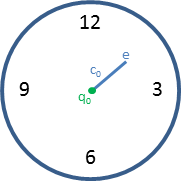
\includegraphics[]{watchcine}
  \caption{
          \textit{La grande aiguille de la montre est une cha\^ine cin\'ematique compos\'ee d'une seule barre rigide.}}
		   \label{watchcine}
\end{figure}

\begin{figure}[htb]
  \centering
    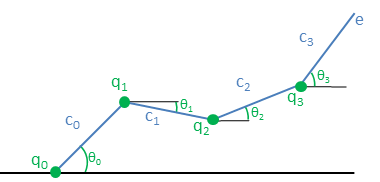
\includegraphics[]{chainangles}
  \caption{
          \textit{Une chaine cin\'ematique compos\'ee de quatre corps rigides.}}
		   \label{chainangle}
\end{figure}

\subsubsection*{Cin\'ematique directe}
Dans un probl\`eme de cin\'ematique directe, on cherche \`a d\'eterminer la position de l'effecteur $e$ en fonction
des valeurs d'angles $\theta_i$ de la cha\^ine cin\'ematique.

On veut donc trouver la fonction $f$ telle que:

\begin{displaymath}  
f\begin{pmatrix} \theta_0 \\ ... \\ \theta_{n-1} \end{pmatrix} = \begin{pmatrix}
x_e \\
y_e
\end{pmatrix}
\end{displaymath}
 
 \subsubsection*{Cin\'ematique inverse}
Dans un probl\`eme de cin\'ematique inverse, on cherche \`a d\'eterminer une combinaison de valeurs d'angles $\theta_i$ qui permette
d'atteindre la position $\begin{pmatrix} x_e \\ y_e \end{pmatrix}$.

On veut donc trouver la fonction $f^{-1}$ telle que:

\begin{displaymath}  
f^{-1} \begin{pmatrix} x_e \\ y_e \end{pmatrix} =  \begin{pmatrix} \theta_0 \\ ... \\ \theta_{n-1} \end{pmatrix}
 \end{displaymath}
 
 Le probl\`eme est que, dans les cas complexes, f n'est pas bijective:
 \begin{itemize}
 \item elle n'est pas surjective car $f^{-1}$ n'est pas forc\'ement d\'efinie partout (figure \ref{outareach});
 \item elle n'est pas injective car il peut exister plusieurs solutions qui permettent d'atteindre la position
 $\begin{pmatrix} x_e \\ y_e \end{pmatrix}$(figure \ref{multisol}).
 \end{itemize}
 
 
 \begin{figure}[htb]
  \centering
    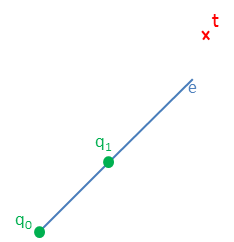
\includegraphics[]{outareach}
  \caption{
          \textit{Le point $t$ ne peut \^etre atteint par l'effecteur $e$.}}
		   \label{outareach}
\end{figure}
 
 
 \begin{figure}[htb]
  \centering
    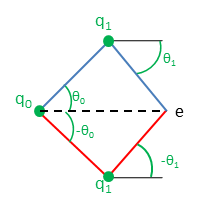
\includegraphics[]{multisol}
  \caption{
          \textit{Diff\'erentes combinaisons d'angles peuvent aboutir \`a la m\^eme position pour l'effecteur $e$.}}
		   \label{multisol}
\end{figure}

Quand une cha\^ine cin\'ematique est trop complexe, il est difficile, voire impossible de d\'efinir correctement $f^{-1}$; c'est pour
cela que des m\'ethodes num\'eriques ont \'et\'e mises au point pour calculer les valeurs de $f^{-1}$, comme la m\'ethode CCD.
  
\subsection{Cin\'ematique en 3 dimensions}
Nous avons vu qu'en deux dimensions nous consid\'erons des rotations autour de l'axe $\vec{Oz} = \vec{Ox} \wedge \vec{Oy}$.
En 3 dimensions, il nous faudra \'egalement consid\'erer des rotations autour des axes $\vec{Ox}$ et $\vec{Oy}$ (figure \ref{rot3d}).
En th\'eorie cela fait donc 3 fois plus d'angles \`a prendre en compte!

Une autre mani\`ere de voir les choses est ramener la combinaison de 3 rotations \`a une seule rotation d'angle $\theta$ autour
d'un axe $\vec{u}$ \`a d\'efinir. Comme pour le cas 2d, \'etant donn\'es 2 vecteurs $\vec{a}$ et $\vec{b}$ $\vec{u}$ se calcule gr\^ace au produit vectoriel:

\begin{displaymath}
\vec{u} = \vec{a} \wedge \vec{b}
\end{displaymath}

Ceci est illustr\'e par la figure \ref{rot3dUnAxe}.

 \begin{figure}[htb]
  \centering
    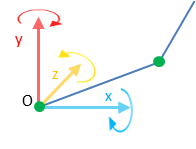
\includegraphics[]{rot3d}
  \caption{
          \textit{Articulation en 3 dimensions: 3 rotations sont possibles.}}
		   \label{rot3d}
\end{figure}
 
  \begin{figure}[htb]
  \centering
    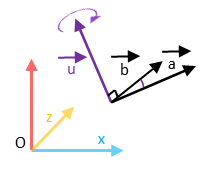
\includegraphics[]{rot3dUnAxe}
  \caption{
          \textit{La transformation permettant d'aligner $\vec{a}$ \`a $\vec{b}$ peut s'exprimer comme une seule rotation autour de l'axe $\vec{u}$.}}
		   \label{rot3dUnAxe}
\end{figure}
 
% Nous allons voir qu'en pratique avec l'algorithme 
% CCD, et gr\^ace aux fonctionalit\'es de |Unity| passer de la 2d \`a la 3d est trivial.
 
\section{L'algorithme CCD}
\label{algo}

\subsection*{D\'efinitions}
\begin{itemize}
\item $p_i$ est la position d'une articulation $q_i$;
\item $p_e$ est la position de l'effecteur;
\item $p_t$ est la position de la cible \`a atteindre.
\end{itemize}


\DeleteShortVerb{|}

\subsection*{D\'eroulement de l'algorithme}
La figure \ref{CCDALL} illustre le d\'eroulement de l'algorithme.
On commence par choisir l'articulation $q_i = q_{n-1}$ la plus proche de l'effecteur.
\begin{itemize}
\item On calcule l'angle $\alpha$ form\'e entre les vecteurs $\vec{q_ip_e}$ et $\vec{q_ip_t}$;
\item On effectue la rotation de centre $p_i$ et d'angle $\alpha$ qui aligne $\vec{q_ip_e}$ et $\vec{q_ip_t}$, autour de l'axe $\vec{q_ip_e} \wedge \vec{q_ip_t}$;
\item Si la distance entre l'effecteur et la cible $||\vec{p_ep_t}||$ est inf\`erieure \`a un nombre $\epsilon \in R$, on arr\^ete l'algorithme, car l'objectif est atteint;
\item Sinon deux cas sont possibles:
	\begin{itemize}
	\item si $i > 1$, on r\'ep\`ete ces op\'erations avec l'articulation $q_{i-1}$;
	\item sinon nous sommes arriv\'es \`a la racine; on recommence alors avec $q_{n-1}$.
	\end{itemize}
\end{itemize}


\MakeShortVerb{|}

   \begin{figure}[htb]
  \centering
    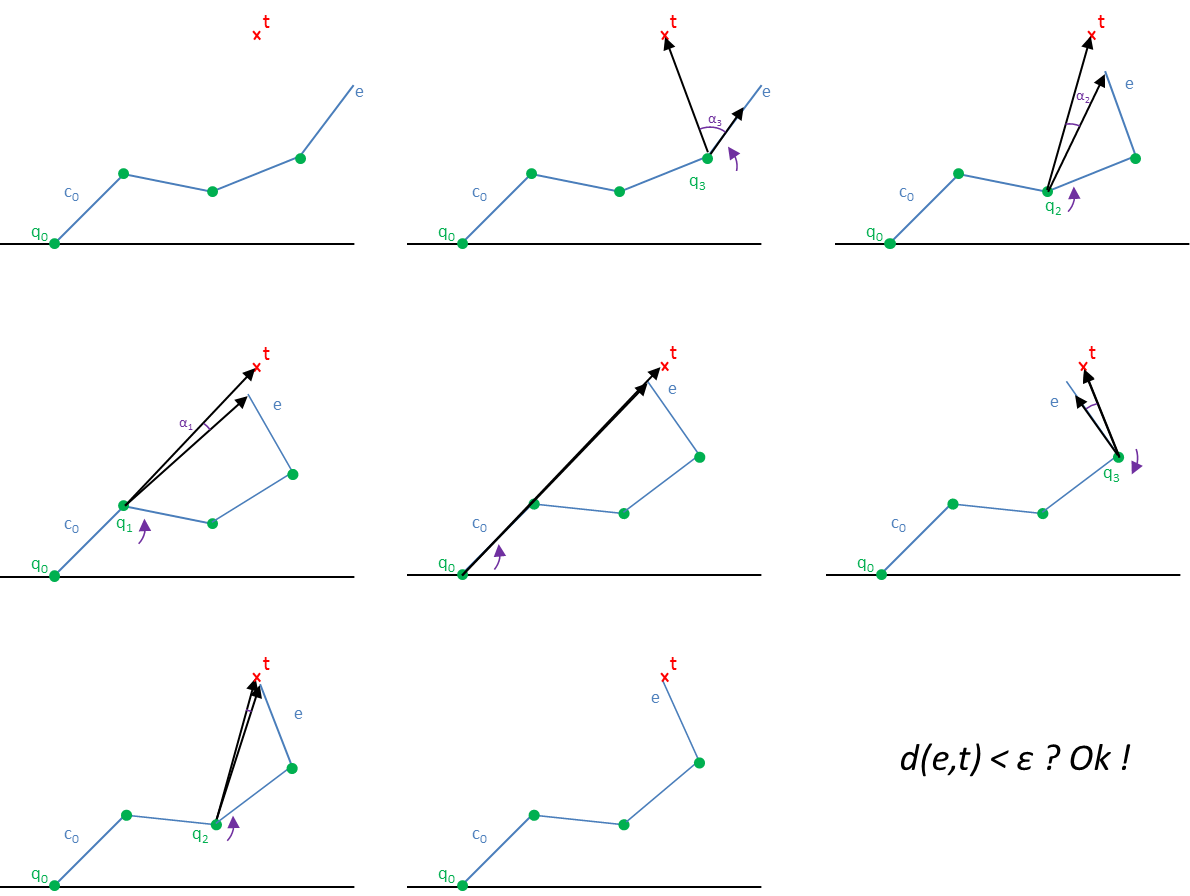
\includegraphics[width=1\linewidth]{CCDALL}
  \caption{
          \textit{Un exemple d'application du CCD en 2 dimenstions. 6 rotations sont n\'ecessaires pour atteindre la cible t.}}
		   \label{CCDALL}
\end{figure}


\section{Questions}
\label{implementation}

\question{1.}Charger la sc\`ene testScene.unity. Depuis l'explorateur de projet, ouvrir le fichier |CCD2d.cs|. Au besoin, regarder
la documentation pour comprendre le type des param\`etres du script, ainsi que ceux pass\'es \`a la m\'ethode |CCDStep2D|.\newline


\question{2.}Ecrire le code de la m\'ethode |ComputeAngle2D| qui calcule un angle sign\'e entre deux |Vector2|. Au besoin se servir de la documentation
de |Vector2| et du namespace |Mathf|.\newline

\question{3.}La m\'ethode |Update| va \^etre appel\'ee une fois par frame. Elle appelle \`a son tour la m\'ethode |CCDStep2D|. C'est une m\'ethode r\'ecursive dans le sens o\`u elle se rappelle elle-m\^eme
avec le parent de l'articulation courante (|joint| en anglais). \\
En d\'eduire ce que repr\'esente |gameObject|, et attacher le script \`a cet objet dans la sc\`ene depuis la fen\^etre |inspector| de |Unity|. \\
Une fois ceci fait, assigner l'objet |target| en tant que param\`etre du script. \newline

\question{4.}Ecrire le code de la m\'ethode |CCDStep2D|. S'aider de la documentation de la classe |Transform| afin de trouver la m\'ethode qui permet
d'effectuer une rotation autour d'un axe. \\
Dans la description de l'algorithme il est dit que l'on arr\^ete l'algorithme si la distance entre l'effecteur et la cible $||\vec{p_ep_t}||$ est inf\`erieure \`a un nombre $\epsilon \in R$.
Il n'y a pas besoin de tester cette condition ici. Pourquoi supprimer cette condition d'arr\^et n'est pas dangereux dans notre cas? \newline

\question{5.}
Lancer l'application. D\'eplacer le cube cible avec les fl\`eches directionelles. V\'erifier que votre impl\'ementation fonctionne. \newline

\question{6.}
Depuis l'|inspector| d\'esactiver le script |CCD2d.cs|. \\ Ajouter le script |CCD3d.cs| au bon objet de la sc\`ene.\\
Ecrire le code manquant pour faire fonctionner le script |CCD3d.cs| en s'aidant de la documentation de la classe |Vector3|.
Constater que sous |Unity| il est encore plus facile de travailler en 3d qu'en 2d :). \newline


\question{7.}
Lancer l'application. Les touches |V| et |B| permettent de d\'eplacer le cube le long de l'axe $\vec{Oz}$, vous permettant de tester votre 
algorithme en 3 dimensions.
\end{document}